\chapter{Using Text Similarity to Detect Social Interactions not Captured by Formal Reply Mechanisms}
\label{ch:reactions}

Studies on social networks often use actions people take on other people's online content as evidence of social interactions for developing their models. In domains including Usenet \cite{Joyce2006}, Wikipedia \cite{Black2011}, and Facebook \cite{Gilbert2009}, explicit replies are interpreted as evidence of interpersonal interaction and social ties.  These explicit reactions are also used in studies of influence online, such as predicting when an item is likely to be forwarded in Twitter (e.g., \cite{Suh2010,Comarela2012}).

Not all responses, however, are explicitly marked by the system.  For instance, a post that is explicitly threaded as a reply to a particular post in a discussion forum might nevertheless address another post or posts.  In Twitter, one of the study cases of this thesis, there are buttons for replying to and retweeting another user's tweet---but users might compose a new tweet that references another recently seen without hitting the reply button.  Users might do this for a variety of reasons, from being inspired to write their own post on a topic they see coming up in their feed to using the system in ways not intended by the designer (such as copying and pasting content into a new tweet rather than pressing a retweet button).  

Being able to identify these non-obvious, indirect responses might allow researchers to have a more accurate view of social interaction than explicit mechanisms provide.  This might also improve overall estimates of users' responsiveness to others, for instance,
at the individual level, they might indicate how desirable a user is as a follower: people might wish to have followers who are more likely to redistribute their content.  Aggregating responsiveness of a user's followers at the ego network level could support better estimates of an individual's potential reach or influence \cite{Domingos2001} based on the responsiveness of their followers.  Better responsiveness measures could also improve transmission probabilities in epidemiology-inspired models of diffusion in social networks \cite{Bakshy2012a}. 

This chapter assesses the prevalence of non-explicit responses in a dataset drawn from Twitter \cite{BarbosaNeto2013, Barbosa}. It is proposed a measure of normalized textual similarity between a user's tweets and recent friends' tweets based on $tf\mhyphen idf$ scores.  Comparing this to the explicit responses provided by the system shows that explicit indicators of response (replies and retweets) in Twitter are in fact associated with high normalized similarity scores.  Choosing conservative score cutoffs for predicting that a tweet is a response and manually inspecting high-scoring tweets that are not marked as responses suggests that explicit indicators miss at least \highNonTaggedTweetCountPct{}\% of reactions. 
Furthermore, this varies between users: some users systematically fail to use formal response mechanisms, meaning that these users are under-represented in studies that rely on explicit indicators of response and under-counted when considering their potential as information spreaders. These results show that the problem of non-explicit responses is an important one with practical implications for understanding interaction and influence online. 
Later work \cite{taxidou2016} studies a similar problem of identifying implicit responses from a provenance point of view. It uses a similar tf-idf method \cite{de2015}, although considering a more holistic approach in contrast with a ego-network, user-centered approach. We discuss the similarities and the results of both methods.


\section{Related Work}

This question of identifying when a user is reacting to some other users' content can be considered a dual 
question to ``is the user going to react to this message'', a question often asked in studies around influence online. 
The usual approach to the latter question is to identify relevant message or network features in the set of (message, reaction), where the reactions are those tagged by the system (e.g., explicit retweets and/or replies in Twitter).  
Using these features, it is possible to build models that predict the likelihood of a reaction given a message.

Such studies often focus on computational models for predicting retweet behavior.  
For instance, Suh et al. \cite{Suh2010} apply Principal Component Analysis to decompose tweets into a space of characteristics, showing that URLs, hashtags, the number of followers and followees, and the age of the account are correlated with retweet behavior. 
Comarela et al. \cite{Comarela2012} also find that previous responses to the same tweeter, the tweeter's sending rate, and the age of a tweet influence retweeting, proposing two ranking methods for reordering tweets to increase retweeting.  
Petrovic et al. \cite{Petrovic2011} built a \textit{passive-aggressive} classifier for answering that took into consideration social characteristics of the tweets' author as well as tweets' textual features, finding that social features are more informative.  
Peng et al. \cite{Peng2011} used \textit{Conditional Random Fields} to model the probability of how a user retweets a message. 

Other studies look at variations of the problem.  
Artzi et al. \cite{Artzi2012} applied \textit{Multiple Additive Regression-Trees} and \textit{Maximum Entropy Classifiers} to predict both retweets and replies, while Hong et al. \cite{Hong2011} model both the binary question of whether a tweet would be retweeted and the eventual number of retweets a message might accrue.  
Luo et al. \cite{Luo2013} and Wang et al. \cite{Wang2012} approach a similar problem: given a user and their followers, who will retweet a message generated by the user?  Both created classifiers to predict the followers that would retweet a message.  
Liu et al. \cite{Liu2013} studied the social network of questions and answers in \textit{Sina Weibo} looking for characteristics that are associated with a higher number of answers.

These prior works identify a number of useful features that researchers often take into consideration when developing their models.  These include textual features of Tweets, user preferences or characteristics, and features of users' networks including pairwise relationships and graph structure.  Table \ref{tab:characteristics} presents a number of these features and the papers that have used them in response prediction.  This thesis focus on the prevalence of implicit responses and complements these works by identifying tweets that, although not marked as a response, are in fact likely to be real responses.  Such tweets would appear as errors or noise to these models; methods for identifying them might improve both these models and our understanding of why these features matter. For instance, account age might turn out to predict retweet behavior mostly because more experienced users are simply more likely to press the retweet button than new users, rather than having a higher innate propensity to retweet.

%% DC 24: Would still like to see at least some meaningful sorting, even if there aren't subheaders.  Right now it's just a big unordered list, which is not helpful.
\begin{table}[htbp]
	\centering
	\tabcolsep=0.11cm
	\singlespacing
	\fontsize{9pt}{10pt}\selectfont
	\begin{tabular}{|>{\raggedright\centering\arraybackslash}m{4cm}|m{11cm}|}
		\hline
		\textbf{Characteristic} & \centering\arraybackslash \textbf{Description} \\ \hline
		URL 																								& Presence of a link in a tweet. \cite{Artzi2012,Comarela2012,Peng2011,Petrovic2011,Suh2010} \\ \hline
		Number of hashtags 																	& Number of hashtags in a tweet. \cite{Artzi2012,Comarela2012,Peng2011,Petrovic2011} \\ \hline
		Number of mentions 																	& Number of mentions in a tweet. \cite{Artzi2012,Comarela2012,Liu2013,Peng2011,Petrovic2011,Suh2010} \\ \hline
		Number of followers 																& Number of followers of the author. \cite{Artzi2012,Hong2011,Liu2013,Luo2013,Petrovic2011,Suh2010,Wang2012} \\ \hline
		Number of followees 																& Number of followees of the author. \cite{Artzi2012,Hong2011,Luo2013,Petrovic2011,Suh2010,Wang2012} \\ \hline
		Presence in lists 																	& Number of times that an author has been added to lists. \cite{Luo2013,Petrovic2011} \\ \hline
		Verified 																						& If the author has a verified account. \cite{Luo2013,Petrovic2011} \\ \hline
		Ratio of followers over followees												& Ratio $followers/followees$ or its inverse. \cite{Artzi2012,Peng2011} \\ \hline
		N-grams 																						& Presence of possible n-grams in the text. Usually used together with dimensionality reduction methods. \cite{Artzi2012,Petrovic2011} \\ \hline
		Number of Stop Words 																& Number of stop words in the tweet. \cite{Artzi2012} \\ \hline
		Time 																								& Time when the user received the tweet. \cite{Artzi2012,Liu2013} \\ \hline
		Day of week 																				& Day of the week when the user received the tweet. \cite{Artzi2012} \\ \hline
		Time zone 																					& If the author and the receiver of a tweet are in the same time zone. \cite{Luo2013} \\ \hline
		Wait time 																					& Average time a user takes to reply or retweet a message. \cite{Comarela2012,Hong2011} \\ \hline
		Timeline position 													& How many messages on average a user receives between receiving and replying (or retweeting) a tweet. \cite{Comarela2012} \\ \hline
		Tweet age 																					& When the tweet being retweeted was originally created. \cite{Comarela2012,Hong2011} \\ \hline
		Previous interaction 																& If the user has already replied to or retweeted the author in the past. \cite{Comarela2012,Luo2013,Wang2012} \\ \hline
		Author's activity 																	& Absolute number, frequency, or distribution that represents how the author tweets. \cite{Comarela2012,Hong2011,Liu2013,Luo2013,Peng2011,Petrovic2011,Suh2010,Wang2012} \\ \hline
		Followees activity 																	& Absolute number, frequency, or distribution that represents how the followees of the user tweet. \cite{Peng2011} \\ \hline
		Tweet size 																					& Number of characters of the tweet. \cite{Comarela2012,Petrovic2011} \\ \hline
		Author's PageRank 																	& PageRank of the author. \cite{Hong2011,Wang2012} \\ \hline
		Reciprocal links 
																		& If the author and the user follow each other. \cite{Hong2011,Peng2011,Wang2012} \\ \hline
		Reciprocal followers 																& Number of followers that the author and the user share. \cite{Peng2011,Wang2012} \\ \hline
		Reciprocal followees 																& Number of followees that the author and the user share. \cite{Peng2011,Wang2012} \\ \hline
		Reciprocal mentions 																& Number of tweets where the author mentions the user or the user mentions the author. \cite{Peng2011} \\ \hline
		Reciprocal retweets 																& Number of retweets that the author and the user share. \cite{Peng2011} \\ \hline
		Clustering coefficients 															& Clustering coefficients of the network structure. \cite{Hong2011} \\ \hline
		Previously retweeted message 												& If and how many times a message has been retweeted by other users in the past. \cite{Hong2011,Suh2010} \\ \hline
		Author's retweet count 															& How many messages of the author have been previously retweeted. \cite{Hong2011,Peng2011} \\ \hline
		Emoticons					 												& If there is an emoticon in the tweet. \cite{Liu2013} \\ \hline
		Message topic 																			& Topic identification on the message text or topic similarity measures between the author's interests and the message topic. \cite{Liu2013,Luo2013,Peng2011,Wang2012} \\ \hline
		Language 																						& User's profile language. \cite{Petrovic2011,Wang2012} \\ \hline
		Favorite 																						& If the tweet has been marked as a favorite by the author. \cite{Petrovic2011,Suh2010} \\ \hline
		Response 																						& If the message received is an answer to a previous message. \cite{Petrovic2011} \\ \hline
		Account age 																				& Age of the tweet author's account. \cite{Suh2010,Wang2012} \\ \hline
		Trending topics words 															& If the tweet has \textit{trending topics}' terms. \cite{Petrovic2011} \\ \hline
		Reciprocal hashtags 																& Number of hashtags in common that the author and the user shared in the past. \cite{Wang2012} \\ \hline
		Reciprocal URLs																			& Number of URLs in common that the author and the user shared in the past. \cite{Wang2012} \\ \hline
		Number of lists																			& Number of lists that an author created. \cite{Wang2012} \\ \hline
	\end{tabular}
	\caption{Some characteristics from online social networks that are commonly used to model users' behavior.} 
	\label{tab:characteristics}
\end{table}

When trying to identify non-explicit responses, having a model that explains which messages a user is most likely to be interested can be valuable; that is, the problem of understanding these (message, user) relationships is related to the problem of understanding the (message, reaction) relationships.  
The main stream of research related to modeling user interests in Twitter is the feed personalization problem, defined by Berkovsky et al. \cite{Berkovsky2015} as creating mechanisms that promote and optimize exhibition of interesting content (messages or people, for instance) according to each user's particular preferences and context.  
In their survey, approaches to feed personalization are divided in three main groups: approaches that consider the pairwise relationship between author and consumer of content, approaches that take into consideration the graph structure of the social network, and approaches that deal with textual information from the users.

As with studies of retweet prediction, feed personalization approaches often use indicators of tie strength as proxies for potential interest.  
Schaal et al. \cite{Schaal2012} measure pairwise user similarity through tf vectors and topic similarity using LDA. 
Goyal et al. \cite{Goyal2010} estimate pairwise influence probability based on the user activity (action log).  There are a wide variety of such features; Gilbert and Karahalios \cite{Gilbert2009} estimate pairwise tie strength based on Facebook data based on over 70 features in categories including intensity, intimacy, duration, reciprocal services, structural, emotional support, and social distance.  

Network structure also plays an important role in feed personalization.  
Uysal et al. \cite{Uysal2011} developed a personalized tweet ranking method based on a retweet metric, useful in reordering feeds or distributing items to users more likely to retweet. 
Paek et al. \cite{Paek2010} asked Facebook users about the perceived importance of items in their timeline, developed classifiers to identify important messages and friends, and studied the predictive power of a number of features including likes, number of comments, presence of links and images, textual information, and shared background information. 
Both the tie strength and network structure approaches rely on explicit interaction as a tool for estimating tie strength; just as with retweet prediction, being able to identify non-explicit responses might improve these models.

Most related to this work are text-focused approaches.  Text is commonly used in feed personalization, by comparing content similarity of Tweets or users to a user's previous activity.  
Hannon et al. \cite{Hannon2011} developed a system for follower recommendation on Twitter based on $tf\mhyphen idf$ similarity between the users' newsfeeds. 
Burgess et al. \cite{Burgess2013} propose a system to automatically select users when creating lists. The method adopts $tf\mhyphen idf$ to compare content users generated, among other measures and evaluates the performance comparing user-made lists with those generated by the system.  This work informs ours by providing evidence that $tf\mhyphen idf$-based methods are useful in understanding attention and interest.

\section{Twitter Dataset}

To study potential responses of social network users we take an approach that considers the information users receive and emit. This allows ego networks to be collected rather than full network data.  
This is often a more feasible approach when dealing with online social networks, since even friendly APIs normally impose rate limits.  
Ego networks are often useful for studying interaction and influence \cite{Welser2011,Sharma2013}; here, they are appropriate because the method requires only a user's content and his followees' in order to reconstruct the feed windows.

%% DC 24: Okay, trying one more tweaking, but not complete rewriting, of this.
The dataset explored in this chapter was collected as part of a project to investigate differences in online behavior between political groups, driven by observations that, in the U.S. 2012 presidential election, Democrats were more active and effective in social media than Republicans.  This work draws on that dataset, using ego networks on Twitter belonging to users that followed Barack Obama crawled in the first three weeks of December 2012 using V1.0 of the Twitter API.

\subsection{IBM Internship}

The author prepared this dataset during his internship at IBM Research Brazil with the co-advisorship of Dr. Claudio Pinhanez. During the extent of the internship, this dataset served as basis for other works in collaboration with IBM's researchers on the fields of agent-based simulations and information diffusion. More specifically, we built a system that would take the network structure as an oriented graph where users are nodes and edges are ``following'' relationships, as well as the messages that were sent though these edges. We then performed a sentiment classification on these messages regarding two topics: Barack Obama and Mitt Romney. Based on each node sentiment emission distribution over the topics and a message's forwarding probability given it was received by one of its peers, we simulated the diffusion and prevalence of such messages on the network. We estimated how the volume of such messages would evolve over time for the whole network, as well as the proportions of positive and negative messages for each of the topics \cite{Gatti2013a, Gatti2013, BarbosaNeto2013}.

While the experiments showed promising venues of how simulation approaches help us to understand diffusion and sentiment propagation in a network, they do not consider implicit reactions of users and non-explicit behavior, subjects that are the focus of this thesis. Also, while the author participated actively in the crawling and initial analysis, most of the simulation approach and models used were contributions of the IBM's researchers. Therefore we chose to highlight these as part of the contribution to the scientific community as an unfolding of the author's Ph.D. trajectory, but not include their full content on the thesis.


\subsection{Crawler's technical aspects}


The crawler first got all the followers for Obama's account, then filtered out users that did not choose English as their profile language or had no tweets in the last month.  It then randomly selected 547 users and collected up to one month (or the Twitter limit of 3200 historical tweets) of Tweets from each user and all of their followees, creating a set of ego networks.

Because of the 3200 tweet per-user limit, as well as occasional API or network errors, the dataset does not contain a complete record of all followees' tweets.  This could affect estimates of the presence of non-explicit responses; thus, networks where a significant proportion of followees' tweets appeared to be missing were filtered out.  Tweets were considered missing when a followee's activity only partially overlapped with the ego user's\footnote{There is a parallel, opposite problem for users who added followees during the ego user's activity period; windows for tweets before the followee was added will incorrectly contain their tweets, which the user could not have responded to.  We saw no good way to address this and so tolerate the error.}, with the number of missing tweets estimated based on the length of overlap and the rate of that followee's tweets.  Users for whom over 20\% of their followers' tweets were estimated missing were removed from the dataset, leaving \totalUsers{} ego networks\footnote{Other thresholds (5\%, 10\%, 50\%, 80\%, 100\%) were tested.  Lower values lead to similar results, while higher values increased the number of users that lacked data for analysis; 20\% was chosen as a reasonable trade-off between sample size and meaningfulness of results.}.


\section{Reaction Identification}

This section presents the definition of the problem and the method used to attack the identification of non-explicit reactions in Twitter.

When users decide to post a message in Twitter, they might be reacting to some content they saw from one of their followees. The first assumption is that the evidence for these reactions are the textual features in a given tweet by user $u$ and textual features in the set of recent tweets by $u$'s followees. Another assumption is that, if $u$ tweeted in reaction to a followee's message, there should be higher text similarity between that tweet and that message. This work focus on text features, rather than user or network characteristics found in prior work, because they have been shown to be useful while simplifying data collection, computation, and modeling.

This leads to this chapters's first research question (\ResearchQuestion\label{rq:similarityPotential}), about whether text similarity has potential for identifying non-explicit responses. 
Do explicit responses in fact tend to have high text similarity? If so, what fraction of high-scoring tweets are non-explicit?  And, even when similarity is lower, when might non-explicit responses be present?

The second research question (\ResearchQuestion\label{rq:usersDistribution}) asked is how these non-explicit responses are distributed among users.  Are many users ``invisible'' because, although they appear to be responsive based on scores, their responses are not explicit?  Why are they lost?  Are they naive or low-frequency users who do not know better than to retype or cut and paste or restate? And, is this likely to be important in estimating the overall responsiveness of users?

\subsection{Influence Window}

The information Twitter presents to a user is the set of tweets sent by their followees in reverse chronological order. Comarela et al. \cite{Comarela2012} study how far back in the user feed is a tweet when replied or retweeted. They divided the users into four sets of increasing levels of activity and found that over 80\% of replies and 60\% of retweets are responses to one of the 50 most recent tweets in a user's feed. They also present cumulative distributions of these replied and retweeted tweets when varying the position in the feed, and the last 100 tweets in the feed contain more than 80\% of the tweets in these distributions.  
Based on this, a window $w_i$ for the tweet $t_i$ is defined as the last $n=100$ tweets generated by user's $u$ followees $f_i$ immediately before $t_i$, taken in reverse chronological order.
Figure \ref{fig:fig_window_explanation} illustrates the window. 

\begin{figure}[!htbp]
\centering
\fontsize{9pt}{10pt}\selectfont
% Graphic for TeX using PGF
% Title: C:\sam\Dropbox\Usp\phd\escience2015\draft01\figures\[scale=0.80]fig_window_explanation.dia
% Creator: Dia v0.97.2
% CreationDate: Mon Mar 09 23:48:24 2015
% For: Samuel
% \usepackage{tikz}
% The following commands are not supported in PSTricks at present
% We define them conditionally, so when they are implemented,
% this pgf file will use them.
\ifx\du\undefined
  \newlength{\du}
\fi
\setlength{\du}{15\unitlength}
\begin{tikzpicture}[scale=0.8]
\pgftransformxscale{1.000000}
\pgftransformyscale{-1.000000}
\definecolor{dialinecolor}{rgb}{0.000000, 0.000000, 0.000000}
\pgfsetstrokecolor{dialinecolor}
\definecolor{dialinecolor}{rgb}{1.000000, 1.000000, 1.000000}
\pgfsetfillcolor{dialinecolor}
\pgfsetlinewidth{0.100000\du}
\pgfsetdash{}{0pt}
\pgfsetdash{}{0pt}
\pgfsetmiterjoin
\definecolor{dialinecolor}{rgb}{0.000000, 0.000000, 0.000000}
\pgfsetstrokecolor{dialinecolor}
\draw (2.653020\du,-4.578300\du)--(2.653020\du,3.865635\du)--(13.062939\du,3.865635\du)--(13.062939\du,-4.578300\du)--cycle;
% setfont left to latex
\definecolor{dialinecolor}{rgb}{0.000000, 0.000000, 0.000000}
\pgfsetstrokecolor{dialinecolor}
\node at (7.857980\du,-0.116333\du){};
\pgfsetlinewidth{0.100000\du}
\pgfsetdash{{1.000000\du}{1.000000\du}}{0\du}
\pgfsetdash{{0.300000\du}{0.300000\du}}{0\du}
\pgfsetmiterjoin
\pgfsetbuttcap
\definecolor{dialinecolor}{rgb}{0.000000, 0.000000, 0.000000}
\pgfsetstrokecolor{dialinecolor}
\pgfpathmoveto{\pgfpoint{2.400000\du}{-13.600000\du}}
\pgfpathcurveto{\pgfpoint{2.400000\du}{-16.200000\du}}{\pgfpoint{13.200000\du}{-16.200000\du}}{\pgfpoint{13.200000\du}{-13.600000\du}}
\pgfpathcurveto{\pgfpoint{13.200000\du}{-11.000000\du}}{\pgfpoint{2.400000\du}{-11.000000\du}}{\pgfpoint{2.400000\du}{-13.600000\du}}
\pgfusepath{stroke}
\pgfsetlinewidth{0.100000\du}
\pgfsetdash{}{0pt}
\pgfsetdash{}{0pt}
\pgfsetbuttcap
{
\definecolor{dialinecolor}{rgb}{0.000000, 0.000000, 0.000000}
\pgfsetfillcolor{dialinecolor}
% was here!!!
\pgfsetarrowsend{latex}
\definecolor{dialinecolor}{rgb}{0.000000, 0.000000, 0.000000}
\pgfsetstrokecolor{dialinecolor}
\draw (7.054030\du,-9.400460\du)--(4.412435\du,-12.796051\du);
}
\pgfsetlinewidth{0.100000\du}
\pgfsetdash{}{0pt}
\pgfsetdash{}{0pt}
\pgfsetbuttcap
{
\definecolor{dialinecolor}{rgb}{0.000000, 0.000000, 0.000000}
\pgfsetfillcolor{dialinecolor}
% was here!!!
\pgfsetarrowsend{latex}
\definecolor{dialinecolor}{rgb}{0.000000, 0.000000, 0.000000}
\pgfsetstrokecolor{dialinecolor}
\draw (7.407290\du,-9.467540\du)--(6.959627\du,-12.635518\du);
}
\pgfsetlinewidth{0.100000\du}
\pgfsetdash{}{0pt}
\pgfsetdash{}{0pt}
\pgfsetbuttcap
{
\definecolor{dialinecolor}{rgb}{0.000000, 0.000000, 0.000000}
\pgfsetfillcolor{dialinecolor}
% was here!!!
\pgfsetarrowsend{latex}
\definecolor{dialinecolor}{rgb}{0.000000, 0.000000, 0.000000}
\pgfsetstrokecolor{dialinecolor}
\draw (7.760560\du,-9.400460\du)--(11.165045\du,-12.864822\du);
}
% setfont left to latex
\definecolor{dialinecolor}{rgb}{0.000000, 0.000000, 0.000000}
\pgfsetstrokecolor{dialinecolor}
\node[anchor=west] at (8.908270\du,-13.424100\du){. . .};
\pgfsetlinewidth{0.100000\du}
\pgfsetdash{}{0pt}
\pgfsetdash{}{0pt}
\pgfsetmiterjoin
\definecolor{dialinecolor}{rgb}{0.000000, 0.000000, 0.000000}
\pgfsetstrokecolor{dialinecolor}
\pgfpathellipse{\pgfpoint{3.831402\du}{-13.542929\du}}{\pgfpoint{0.923132\du}{0\du}}{\pgfpoint{0\du}{0.881171\du}}
\pgfusepath{stroke}
% setfont left to latex
\definecolor{dialinecolor}{rgb}{0.000000, 0.000000, 0.000000}
\pgfsetstrokecolor{dialinecolor}
\node at (3.831402\du,-13.302929\du){};
% setfont left to latex
\definecolor{dialinecolor}{rgb}{0.000000, 0.000000, 0.000000}
\pgfsetstrokecolor{dialinecolor}
\node[anchor=west] at (3.212350\du,-13.542900\du){$f_1$};
\pgfsetlinewidth{0.100000\du}
\pgfsetdash{}{0pt}
\pgfsetdash{}{0pt}
\pgfsetmiterjoin
\definecolor{dialinecolor}{rgb}{0.000000, 0.000000, 0.000000}
\pgfsetstrokecolor{dialinecolor}
\pgfpathellipse{\pgfpoint{6.831402\du}{-13.542929\du}}{\pgfpoint{0.923132\du}{0\du}}{\pgfpoint{0\du}{0.881171\du}}
\pgfusepath{stroke}
% setfont left to latex
\definecolor{dialinecolor}{rgb}{0.000000, 0.000000, 0.000000}
\pgfsetstrokecolor{dialinecolor}
\node at (6.831402\du,-13.302929\du){};
% setfont left to latex
\definecolor{dialinecolor}{rgb}{0.000000, 0.000000, 0.000000}
\pgfsetstrokecolor{dialinecolor}
\node[anchor=west] at (6.212350\du,-13.542900\du){$f_2$};
\pgfsetlinewidth{0.100000\du}
\pgfsetdash{}{0pt}
\pgfsetdash{}{0pt}
\pgfsetmiterjoin
\definecolor{dialinecolor}{rgb}{0.000000, 0.000000, 0.000000}
\pgfsetstrokecolor{dialinecolor}
\pgfpathellipse{\pgfpoint{11.831432\du}{-13.542929\du}}{\pgfpoint{0.923132\du}{0\du}}{\pgfpoint{0\du}{0.881171\du}}
\pgfusepath{stroke}
% setfont left to latex
\definecolor{dialinecolor}{rgb}{0.000000, 0.000000, 0.000000}
\pgfsetstrokecolor{dialinecolor}
\node at (11.831432\du,-13.302929\du){};
% setfont left to latex
\definecolor{dialinecolor}{rgb}{0.000000, 0.000000, 0.000000}
\pgfsetstrokecolor{dialinecolor}
\node[anchor=west] at (11.137900\du,-13.542900\du){$f_m$};
\pgfsetlinewidth{0.100000\du}
\pgfsetdash{}{0pt}
\pgfsetdash{}{0pt}
\pgfsetmiterjoin
\definecolor{dialinecolor}{rgb}{0.000000, 0.000000, 0.000000}
\pgfsetstrokecolor{dialinecolor}
\pgfpathellipse{\pgfpoint{7.407292\du}{-8.586369\du}}{\pgfpoint{0.923132\du}{0\du}}{\pgfpoint{0\du}{0.881171\du}}
\pgfusepath{stroke}
% setfont left to latex
\definecolor{dialinecolor}{rgb}{0.000000, 0.000000, 0.000000}
\pgfsetstrokecolor{dialinecolor}
\node at (7.407292\du,-8.346369\du){};
% setfont left to latex
\definecolor{dialinecolor}{rgb}{0.000000, 0.000000, 0.000000}
\pgfsetstrokecolor{dialinecolor}
\node[anchor=west] at (6.910820\du,-8.583810\du){$u$};
\pgfsetlinewidth{0.100000\du}
\pgfsetdash{{1.000000\du}{1.000000\du}}{0\du}
\pgfsetdash{{0.300000\du}{0.300000\du}}{0\du}
\pgfsetbuttcap
{
\definecolor{dialinecolor}{rgb}{0.000000, 0.000000, 0.000000}
\pgfsetfillcolor{dialinecolor}
% was here!!!
\pgfsetarrowsend{stealth}
\definecolor{dialinecolor}{rgb}{0.000000, 0.000000, 0.000000}
\pgfsetstrokecolor{dialinecolor}
\pgfpathmoveto{\pgfpoint{2.400279\du}{-13.600459\du}}
\pgfpatharc{212}{147}{12.351908\du and 12.351908\du}
\pgfusepath{stroke}
}
\pgfsetlinewidth{0.100000\du}
\pgfsetdash{}{0pt}
\pgfsetdash{}{0pt}
\pgfsetmiterjoin
\definecolor{dialinecolor}{rgb}{0.000000, 0.000000, 0.000000}
\pgfsetstrokecolor{dialinecolor}
\draw (2.645190\du,-6.869750\du)--(2.645190\du,-4.969750\du)--(13.055109\du,-4.969750\du)--(13.055109\du,-6.869750\du)--cycle;
% setfont left to latex
\definecolor{dialinecolor}{rgb}{0.000000, 0.000000, 0.000000}
\pgfsetstrokecolor{dialinecolor}
\node at (7.850150\du,-5.679750\du){};
\pgfsetlinewidth{0.100000\du}
\pgfsetdash{}{0pt}
\pgfsetdash{}{0pt}
\pgfsetbuttcap
{
\definecolor{dialinecolor}{rgb}{0.000000, 0.000000, 0.000000}
\pgfsetfillcolor{dialinecolor}
% was here!!!
\definecolor{dialinecolor}{rgb}{0.000000, 0.000000, 0.000000}
\pgfsetstrokecolor{dialinecolor}
\draw (2.653020\du,-2.467320\du)--(13.062900\du,-2.467320\du);
}
\pgfsetlinewidth{0.100000\du}
\pgfsetdash{}{0pt}
\pgfsetdash{}{0pt}
\pgfsetbuttcap
{
\definecolor{dialinecolor}{rgb}{0.000000, 0.000000, 0.000000}
\pgfsetfillcolor{dialinecolor}
% was here!!!
\definecolor{dialinecolor}{rgb}{0.000000, 0.000000, 0.000000}
\pgfsetstrokecolor{dialinecolor}
\draw (2.653020\du,-0.356333\du)--(13.062900\du,-0.356333\du);
}
\pgfsetlinewidth{0.100000\du}
\pgfsetdash{}{0pt}
\pgfsetdash{}{0pt}
\pgfsetbuttcap
{
\definecolor{dialinecolor}{rgb}{0.000000, 0.000000, 0.000000}
\pgfsetfillcolor{dialinecolor}
% was here!!!
\definecolor{dialinecolor}{rgb}{0.000000, 0.000000, 0.000000}
\pgfsetstrokecolor{dialinecolor}
\draw (2.653020\du,1.754650\du)--(13.062900\du,1.754650\du);
}
% setfont left to latex
\definecolor{dialinecolor}{rgb}{0.000000, 0.000000, 0.000000}
\pgfsetstrokecolor{dialinecolor}
\node[anchor=west] at (3.278500\du,-5.863530\du){User's $u$ username and tweet $t_i$};
% setfont left to latex
\definecolor{dialinecolor}{rgb}{0.000000, 0.000000, 0.000000}
\pgfsetstrokecolor{dialinecolor}
\node[anchor=west] at (7.857980\du,-0.356333\du){};
% setfont left to latex
\definecolor{dialinecolor}{rgb}{0.000000, 0.000000, 0.000000}
\pgfsetstrokecolor{dialinecolor}
\node[anchor=west] at (4.983670\du,-3.436350\du){Followee tweet $ft_1$};
% setfont left to latex
\definecolor{dialinecolor}{rgb}{0.000000, 0.000000, 0.000000}
\pgfsetstrokecolor{dialinecolor}
\node[anchor=west] at (4.980080\du,-1.418130\du){Followee tweet $ft_2$};
% setfont left to latex
\definecolor{dialinecolor}{rgb}{0.000000, 0.000000, 0.000000}
\pgfsetstrokecolor{dialinecolor}
\node[anchor=west] at (4.991310\du,2.830500\du){Followee tweet $ft_n$};
\pgfsetlinewidth{0.100000\du}
\pgfsetdash{}{0pt}
\pgfsetdash{}{0pt}
\pgfsetmiterjoin
\pgfsetbuttcap
{
\definecolor{dialinecolor}{rgb}{0.000000, 0.000000, 0.000000}
\pgfsetfillcolor{dialinecolor}
% was here!!!
\definecolor{dialinecolor}{rgb}{0.000000, 0.000000, 0.000000}
\pgfsetstrokecolor{dialinecolor}
\pgfpathmoveto{\pgfpoint{13.235600\du}{-4.584360\du}}
\pgfpathcurveto{\pgfpoint{14.235600\du}{-4.724360\du}}{\pgfpoint{13.355600\du}{-0.334364\du}}{\pgfpoint{13.655600\du}{-0.334364\du}}
\pgfpathcurveto{\pgfpoint{13.955600\du}{-0.334364\du}}{\pgfpoint{13.955600\du}{-0.334364\du}}{\pgfpoint{13.655600\du}{-0.334364\du}}
\pgfpathcurveto{\pgfpoint{13.355600\du}{-0.334364\du}}{\pgfpoint{14.145600\du}{4.005640\du}}{\pgfpoint{13.235600\du}{3.865640\du}}
\pgfusepath{stroke}
}
% setfont left to latex
\definecolor{dialinecolor}{rgb}{0.000000, 0.000000, 0.000000}
\pgfsetstrokecolor{dialinecolor}
\node[anchor=west] at (13.848700\du,-0.247892\du){Window $w_i$};
\pgfsetlinewidth{0.100000\du}
\pgfsetdash{{1.000000\du}{1.000000\du}}{0\du}
\pgfsetdash{{0.300000\du}{0.300000\du}}{0\du}
\pgfsetbuttcap
{
\definecolor{dialinecolor}{rgb}{0.000000, 0.000000, 0.000000}
\pgfsetfillcolor{dialinecolor}
% was here!!!
\pgfsetarrowsstart{stealth}
\definecolor{dialinecolor}{rgb}{0.000000, 0.000000, 0.000000}
\pgfsetstrokecolor{dialinecolor}
\pgfpathmoveto{\pgfpoint{10.452600\du}{-6.869748\du}}
\pgfpatharc{357}{262}{1.864634\du and 1.864634\du}
\pgfusepath{stroke}
}
% setfont left to latex
\definecolor{dialinecolor}{rgb}{0.000000, 0.000000, 0.000000}
\pgfsetstrokecolor{dialinecolor}
\node[anchor=west] at (7.275010\du,0.424998\du){.};
% setfont left to latex
\definecolor{dialinecolor}{rgb}{0.000000, 0.000000, 0.000000}
\pgfsetstrokecolor{dialinecolor}
\node[anchor=west] at (7.275010\du,0.724998\du){.};
% setfont left to latex
\definecolor{dialinecolor}{rgb}{0.000000, 0.000000, 0.000000}
\pgfsetstrokecolor{dialinecolor}
\node[anchor=west] at (7.275010\du,1.025000\du){.};
\end{tikzpicture}

\caption{Construction of the window $w_i$ for the tweet $t_i$. The tweets in the window (in this work, $n=100$) are those most generated by user $u$'s followees most recently before $t_i$.} \label{fig:fig_window_explanation}
\end{figure}

\subsection{Textual Features}

Each tweet in a user's feed also carries associated meta-data besides the message itself, such as the author's profile and user name, tweet creation time, number of times liked, and number of times retweeted. In this analysis, users are modeled as primarily paying attention to the textual content when considering a response; thus, only textual features the user's feed exposes are considered.  

Tweets are first preprocessed using Python's NLTK package \cite{Bird2009} to be lower case, remove stopwords, and apply Snowball stemming, all common practices when using $tf\mhyphen idf$ scoring.  Hashtags, usernames, and processed words are then extracted using the regular expressions shown in Table \ref{tab:regularExpressions}.  Finally, the tweet author's username is added as a feature since that is also visible in the feed.

%% DC 16: In general, unless there's a strong IEEE style guideline against it, figures and tables should go at the top or bottom of pages rather than in the middle.
\begin{table}[!tb]
	\fontsize{9pt}{10pt}\selectfont
	\centering
		\begin{tabular}{|l|c|}
			\hline
			Hashtags & \verb!(?:[\s|^])(#[\w]+)! \\ \hline
			Users & \verb!\B(?:[@?])([\w]{1,20})! \\ \hline
			Words & \verb!(?:^|[\s][^@?#\s\w]*)([\w]+)! \\ \hline
		\end{tabular}
		\caption{Regular expressions used to extract features from tweets.}
	\label{tab:regularExpressions}
\end{table}

\subsection{Message Scoring}

\begin{figure}[!tb]
\centering
\fontsize{9pt}{10pt}\selectfont
% Graphic for TeX using PGF
% Title: C:\sam\Dropbox\Usp\phd\escience2015\draft01\figures\[scale=0.80]fig_tfidf_explanation.dia
% Creator: Dia v0.97.2
% CreationDate: Fri Mar 06 00:05:25 2015
% For: Samuel
% \usepackage{tikz}
% The following commands are not supported in PSTricks at present
% We define them conditionally, so when they are implemented,
% this pgf file will use them.
\ifx\du\undefined
  \newlength{\du}
\fi
\setlength{\du}{15\unitlength}
\begin{tikzpicture}[scale=1]
\pgftransformxscale{1.000000}
\pgftransformyscale{-1.000000}
\definecolor{dialinecolor}{rgb}{0.000000, 0.000000, 0.000000}
\pgfsetstrokecolor{dialinecolor}
\definecolor{dialinecolor}{rgb}{1.000000, 1.000000, 1.000000}
\pgfsetfillcolor{dialinecolor}
\pgfsetlinewidth{0.100000\du}
\pgfsetdash{}{0pt}
\pgfsetdash{}{0pt}
\pgfsetmiterjoin
\definecolor{dialinecolor}{rgb}{0.000000, 0.000000, 0.000000}
\pgfsetstrokecolor{dialinecolor}
\draw (27.982000\du,-15.000000\du)--(27.982000\du,-8.000000\du)--(32.582000\du,-8.000000\du)--(32.582000\du,-15.000000\du)--cycle;
% setfont left to latex
\definecolor{dialinecolor}{rgb}{0.000000, 0.000000, 0.000000}
\pgfsetstrokecolor{dialinecolor}
\node at (30.282000\du,-11.374167\du){};
\pgfsetlinewidth{0.100000\du}
\pgfsetdash{}{0pt}
\pgfsetdash{}{0pt}
\pgfsetmiterjoin
\definecolor{dialinecolor}{rgb}{0.000000, 0.000000, 0.000000}
\pgfsetstrokecolor{dialinecolor}
\draw (17.982000\du,-15.050000\du)--(17.982000\du,-14.200000\du)--(22.582000\du,-14.200000\du)--(22.582000\du,-15.050000\du)--cycle;
% setfont left to latex
\definecolor{dialinecolor}{rgb}{0.000000, 0.000000, 0.000000}
\pgfsetstrokecolor{dialinecolor}
\node at (20.282000\du,-14.499167\du){};
\pgfsetlinewidth{0.100000\du}
\pgfsetdash{}{0pt}
\pgfsetdash{}{0pt}
\pgfsetmiterjoin
\definecolor{dialinecolor}{rgb}{0.000000, 0.000000, 0.000000}
\pgfsetstrokecolor{dialinecolor}
\draw (17.982000\du,-14.000000\du)--(17.982000\du,-11.000000\du)--(22.582000\du,-11.000000\du)--(22.582000\du,-14.000000\du)--cycle;
% setfont left to latex
\definecolor{dialinecolor}{rgb}{0.000000, 0.000000, 0.000000}
\pgfsetstrokecolor{dialinecolor}
\node at (20.282000\du,-12.374167\du){$w_1$};
\pgfsetlinewidth{0.100000\du}
\pgfsetdash{}{0pt}
\pgfsetdash{}{0pt}
\pgfsetmiterjoin
\definecolor{dialinecolor}{rgb}{0.000000, 0.000000, 0.000000}
\pgfsetstrokecolor{dialinecolor}
\draw (17.982000\du,-7.922890\du)--(17.982000\du,-4.922890\du)--(22.582000\du,-4.922890\du)--(22.582000\du,-7.922890\du)--cycle;
% setfont left to latex
\definecolor{dialinecolor}{rgb}{0.000000, 0.000000, 0.000000}
\pgfsetstrokecolor{dialinecolor}
\node at (20.282000\du,-6.297057\du){$w_2$};
\pgfsetlinewidth{0.100000\du}
\pgfsetdash{}{0pt}
\pgfsetdash{}{0pt}
\pgfsetmiterjoin
\definecolor{dialinecolor}{rgb}{0.000000, 0.000000, 0.000000}
\pgfsetstrokecolor{dialinecolor}
\draw (17.982000\du,1.000000\du)--(17.982000\du,4.000000\du)--(22.582000\du,4.000000\du)--(22.582000\du,1.000000\du)--cycle;
% setfont left to latex
\definecolor{dialinecolor}{rgb}{0.000000, 0.000000, 0.000000}
\pgfsetstrokecolor{dialinecolor}
\node at (20.282000\du,2.625833\du){$w_m$};
% setfont left to latex
\definecolor{dialinecolor}{rgb}{0.000000, 0.000000, 0.000000}
\pgfsetstrokecolor{dialinecolor}
\node[anchor=west] at (19.913200\du,-3.460260\du){.};
% setfont left to latex
\definecolor{dialinecolor}{rgb}{0.000000, 0.000000, 0.000000}
\pgfsetstrokecolor{dialinecolor}
\node[anchor=west] at (19.913200\du,-2.613593\du){.};
% setfont left to latex
\definecolor{dialinecolor}{rgb}{0.000000, 0.000000, 0.000000}
\pgfsetstrokecolor{dialinecolor}
\node[anchor=west] at (19.913200\du,-1.766927\du){.};
\pgfsetlinewidth{0.100000\du}
\pgfsetdash{}{0pt}
\pgfsetdash{}{0pt}
\pgfsetbuttcap
{
\definecolor{dialinecolor}{rgb}{0.000000, 0.000000, 0.000000}
\pgfsetfillcolor{dialinecolor}
% was here!!!
\pgfsetarrowsend{stealth}
\definecolor{dialinecolor}{rgb}{0.000000, 0.000000, 0.000000}
\pgfsetstrokecolor{dialinecolor}
\draw (22.582000\du,-12.500000\du)--(27.883672\du,-11.518209\du);
}
\pgfsetlinewidth{0.100000\du}
\pgfsetdash{}{0pt}
\pgfsetdash{}{0pt}
\pgfsetbuttcap
{
\definecolor{dialinecolor}{rgb}{0.000000, 0.000000, 0.000000}
\pgfsetfillcolor{dialinecolor}
% was here!!!
\pgfsetarrowsend{stealth}
\definecolor{dialinecolor}{rgb}{0.000000, 0.000000, 0.000000}
\pgfsetstrokecolor{dialinecolor}
\draw (22.582000\du,-6.422890\du)--(27.763434\du,-11.294503\du);
}
\pgfsetlinewidth{0.100000\du}
\pgfsetdash{}{0pt}
\pgfsetdash{}{0pt}
\pgfsetbuttcap
{
\definecolor{dialinecolor}{rgb}{0.000000, 0.000000, 0.000000}
\pgfsetfillcolor{dialinecolor}
% was here!!!
\pgfsetarrowsend{stealth}
\definecolor{dialinecolor}{rgb}{0.000000, 0.000000, 0.000000}
\pgfsetstrokecolor{dialinecolor}
\draw (22.622657\du,2.475543\du)--(27.662785\du,-10.591456\du);
}
% setfont left to latex
\definecolor{dialinecolor}{rgb}{0.000000, 0.000000, 0.000000}
\pgfsetstrokecolor{dialinecolor}
\node at (30.284900\du,-12.120188\du){Set $D$ of };
% setfont left to latex
\definecolor{dialinecolor}{rgb}{0.000000, 0.000000, 0.000000}
\pgfsetstrokecolor{dialinecolor}
\node at (30.284900\du,-11.485187\du){all windows'};
% setfont left to latex
\definecolor{dialinecolor}{rgb}{0.000000, 0.000000, 0.000000}
\pgfsetstrokecolor{dialinecolor}
\node at (30.284900\du,-10.850187\du){tweets without};
% setfont left to latex
\definecolor{dialinecolor}{rgb}{0.000000, 0.000000, 0.000000}
\pgfsetstrokecolor{dialinecolor}
\node at (30.284900\du,-10.215187\du){repetition. };
\pgfsetlinewidth{0.100000\du}
\pgfsetdash{}{0pt}
\pgfsetdash{}{0pt}
\pgfsetmiterjoin
\definecolor{dialinecolor}{rgb}{0.000000, 0.000000, 0.000000}
\pgfsetstrokecolor{dialinecolor}
\draw (27.982000\du,-3.000000\du)--(27.982000\du,4.000000\du)--(32.582000\du,4.000000\du)--(32.582000\du,-3.000000\du)--cycle;
% setfont left to latex
\definecolor{dialinecolor}{rgb}{0.000000, 0.000000, 0.000000}
\pgfsetstrokecolor{dialinecolor}
\node at (30.282000\du,0.625833\du){};
\pgfsetlinewidth{0.100000\du}
\pgfsetdash{{1.000000\du}{1.000000\du}}{0\du}
\pgfsetdash{{0.300000\du}{0.300000\du}}{0\du}
\pgfsetbuttcap
{
\definecolor{dialinecolor}{rgb}{0.000000, 0.000000, 0.000000}
\pgfsetfillcolor{dialinecolor}
% was here!!!
\definecolor{dialinecolor}{rgb}{0.000000, 0.000000, 0.000000}
\pgfsetstrokecolor{dialinecolor}
\draw (27.982000\du,1.400000\du)--(32.582000\du,1.400000\du);
}
\pgfsetlinewidth{0.100000\du}
\pgfsetdash{{0.300000\du}{0.300000\du}}{0\du}
\pgfsetdash{{0.300000\du}{0.300000\du}}{0\du}
\pgfsetbuttcap
{
\definecolor{dialinecolor}{rgb}{0.000000, 0.000000, 0.000000}
\pgfsetfillcolor{dialinecolor}
% was here!!!
\definecolor{dialinecolor}{rgb}{0.000000, 0.000000, 0.000000}
\pgfsetstrokecolor{dialinecolor}
\draw (27.982000\du,3.000000\du)--(32.582000\du,3.000000\du);
}
% setfont left to latex
\definecolor{dialinecolor}{rgb}{0.000000, 0.000000, 0.000000}
\pgfsetstrokecolor{dialinecolor}
\node[anchor=west] at (29.533600\du,2.200000\du){$w_i$};
\pgfsetlinewidth{0.100000\du}
\pgfsetdash{}{0pt}
\pgfsetdash{}{0pt}
\pgfsetbuttcap
{
\definecolor{dialinecolor}{rgb}{0.000000, 0.000000, 0.000000}
\pgfsetfillcolor{dialinecolor}
% was here!!!
\pgfsetarrowsend{stealth}
\definecolor{dialinecolor}{rgb}{0.000000, 0.000000, 0.000000}
\pgfsetstrokecolor{dialinecolor}
\draw (30.232000\du,-8.000000\du)--(30.258686\du,-4.562557\du);
}
% setfont left to latex
\definecolor{dialinecolor}{rgb}{0.000000, 0.000000, 0.000000}
\pgfsetstrokecolor{dialinecolor}
\node at (33.436600\du,-6.301917\du){Generate};
% setfont left to latex
\definecolor{dialinecolor}{rgb}{0.000000, 0.000000, 0.000000}
\pgfsetstrokecolor{dialinecolor}
\node at (33.436600\du,-5.666917\du){tf-idf matrix.};
% setfont left to latex
\definecolor{dialinecolor}{rgb}{0.000000, 0.000000, 0.000000}
\pgfsetstrokecolor{dialinecolor}
\node at (35.638400\du,-2.788980\du){We use the user's};
% setfont left to latex
\definecolor{dialinecolor}{rgb}{0.000000, 0.000000, 0.000000}
\pgfsetstrokecolor{dialinecolor}
\node at (35.638400\du,-2.153980\du){tweet as a query };
% setfont left to latex
\definecolor{dialinecolor}{rgb}{0.000000, 0.000000, 0.000000}
\pgfsetstrokecolor{dialinecolor}
\node at (35.638400\du,-1.518980\du){to search in the };
% setfont left to latex
\definecolor{dialinecolor}{rgb}{0.000000, 0.000000, 0.000000}
\pgfsetstrokecolor{dialinecolor}
\node at (35.638400\du,-0.883980\du){window's tweets for };
% setfont left to latex
\definecolor{dialinecolor}{rgb}{0.000000, 0.000000, 0.000000}
\pgfsetstrokecolor{dialinecolor}
\node at (35.638400\du,-0.248980\du){the most relevant};
% setfont left to latex
\definecolor{dialinecolor}{rgb}{0.000000, 0.000000, 0.000000}
\pgfsetstrokecolor{dialinecolor}
\node at (35.638400\du,0.386020\du){document.};
% setfont left to latex
\definecolor{dialinecolor}{rgb}{0.000000, 0.000000, 0.000000}
\pgfsetstrokecolor{dialinecolor}
\node at (30.243200\du,-2.242481\du){Evaluate the};
% setfont left to latex
\definecolor{dialinecolor}{rgb}{0.000000, 0.000000, 0.000000}
\pgfsetstrokecolor{dialinecolor}
\node at (30.243200\du,-1.607481\du){score in the};
% setfont left to latex
\definecolor{dialinecolor}{rgb}{0.000000, 0.000000, 0.000000}
\pgfsetstrokecolor{dialinecolor}
\node at (30.243200\du,-0.972481\du){window $w_i$.};
% setfont left to latex
\definecolor{dialinecolor}{rgb}{0.000000, 0.000000, 0.000000}
\pgfsetstrokecolor{dialinecolor}
\node at (30.243200\du,-0.337481\du){Normalize by};
% setfont left to latex
\definecolor{dialinecolor}{rgb}{0.000000, 0.000000, 0.000000}
\pgfsetstrokecolor{dialinecolor}
\node at (30.243200\du,0.297519\du){the largest row};
% setfont left to latex
\definecolor{dialinecolor}{rgb}{0.000000, 0.000000, 0.000000}
\pgfsetstrokecolor{dialinecolor}
\node at (30.243200\du,0.932519\du){sum in $w_i$.};
\pgfsetlinewidth{0.100000\du}
\pgfsetdash{{1.000000\du}{1.000000\du}}{0\du}
\pgfsetdash{{0.300000\du}{0.300000\du}}{0\du}
\pgfsetbuttcap
{
\definecolor{dialinecolor}{rgb}{0.000000, 0.000000, 0.000000}
\pgfsetfillcolor{dialinecolor}
% was here!!!
\pgfsetarrowsstart{stealth}
\definecolor{dialinecolor}{rgb}{0.000000, 0.000000, 0.000000}
\pgfsetstrokecolor{dialinecolor}
\pgfpathmoveto{\pgfpoint{32.581740\du}{2.249934\du}}
\pgfpatharc{105}{53}{3.591028\du and 3.591028\du}
\pgfusepath{stroke}
}
% setfont left to latex
\definecolor{dialinecolor}{rgb}{0.000000, 0.000000, 0.000000}
\pgfsetstrokecolor{dialinecolor}
\node[anchor=west] at (19.702600\du,-14.600000\du){$t_1$};
\pgfsetlinewidth{0.100000\du}
\pgfsetdash{}{0pt}
\pgfsetdash{}{0pt}
\pgfsetmiterjoin
\definecolor{dialinecolor}{rgb}{0.000000, 0.000000, 0.000000}
\pgfsetstrokecolor{dialinecolor}
\draw (17.994300\du,-9.000000\du)--(17.994300\du,-8.150000\du)--(22.594300\du,-8.150000\du)--(22.594300\du,-9.000000\du)--cycle;
% setfont left to latex
\definecolor{dialinecolor}{rgb}{0.000000, 0.000000, 0.000000}
\pgfsetstrokecolor{dialinecolor}
\node at (20.294300\du,-8.449167\du){};
% setfont left to latex
\definecolor{dialinecolor}{rgb}{0.000000, 0.000000, 0.000000}
\pgfsetstrokecolor{dialinecolor}
\node[anchor=west] at (19.714900\du,-8.550000\du){$t_2$};
\pgfsetlinewidth{0.100000\du}
\pgfsetdash{}{0pt}
\pgfsetdash{}{0pt}
\pgfsetmiterjoin
\definecolor{dialinecolor}{rgb}{0.000000, 0.000000, 0.000000}
\pgfsetstrokecolor{dialinecolor}
\draw (17.994300\du,-0.100000\du)--(17.994300\du,0.750000\du)--(22.594300\du,0.750000\du)--(22.594300\du,-0.100000\du)--cycle;
% setfont left to latex
\definecolor{dialinecolor}{rgb}{0.000000, 0.000000, 0.000000}
\pgfsetstrokecolor{dialinecolor}
\node at (20.294300\du,0.450833\du){};
% setfont left to latex
\definecolor{dialinecolor}{rgb}{0.000000, 0.000000, 0.000000}
\pgfsetstrokecolor{dialinecolor}
\node[anchor=west] at (19.714900\du,0.350000\du){$t_m$};
\pgfsetlinewidth{0.100000\du}
\pgfsetdash{}{0pt}
\pgfsetdash{}{0pt}
\pgfsetmiterjoin
\definecolor{dialinecolor}{rgb}{0.000000, 0.000000, 0.000000}
\pgfsetstrokecolor{dialinecolor}
\draw (33.343800\du,0.779389\du)--(33.343800\du,1.629389\du)--(37.943800\du,1.629389\du)--(37.943800\du,0.779389\du)--cycle;
% setfont left to latex
\definecolor{dialinecolor}{rgb}{0.000000, 0.000000, 0.000000}
\pgfsetstrokecolor{dialinecolor}
\node at (35.643800\du,1.330222\du){};
% setfont left to latex
\definecolor{dialinecolor}{rgb}{0.000000, 0.000000, 0.000000}
\pgfsetstrokecolor{dialinecolor}
\node[anchor=west] at (34.949800\du,1.229390\du){$t_i$};
\pgfsetlinewidth{0.100000\du}
\pgfsetdash{}{0pt}
\pgfsetdash{}{0pt}
\pgfsetmiterjoin
\pgfsetbuttcap
{
\definecolor{dialinecolor}{rgb}{0.000000, 0.000000, 0.000000}
\pgfsetfillcolor{dialinecolor}
% was here!!!
\definecolor{dialinecolor}{rgb}{0.000000, 0.000000, 0.000000}
\pgfsetstrokecolor{dialinecolor}
\pgfpathmoveto{\pgfpoint{27.800000\du}{-3.000000\du}}
\pgfpathcurveto{\pgfpoint{26.720000\du}{-3.120000\du}}{\pgfpoint{27.600000\du}{0.600000\du}}{\pgfpoint{27.420000\du}{0.600000\du}}
\pgfpathcurveto{\pgfpoint{27.240000\du}{0.600000\du}}{\pgfpoint{27.240000\du}{0.600000\du}}{\pgfpoint{27.420000\du}{0.600000\du}}
\pgfpathcurveto{\pgfpoint{27.600000\du}{0.600000\du}}{\pgfpoint{26.720000\du}{4.100000\du}}{\pgfpoint{27.800000\du}{4.000000\du}}
\pgfusepath{stroke}
}
% setfont left to latex
\definecolor{dialinecolor}{rgb}{0.000000, 0.000000, 0.000000}
\pgfsetstrokecolor{dialinecolor}
\node at (25.470271\du,0.507500\du){$documents$};
\pgfsetlinewidth{0.100000\du}
\pgfsetdash{}{0pt}
\pgfsetdash{}{0pt}
\pgfsetmiterjoin
\pgfsetbuttcap
{
\definecolor{dialinecolor}{rgb}{0.000000, 0.000000, 0.000000}
\pgfsetfillcolor{dialinecolor}
% was here!!!
\definecolor{dialinecolor}{rgb}{0.000000, 0.000000, 0.000000}
\pgfsetstrokecolor{dialinecolor}
\pgfpathmoveto{\pgfpoint{32.580000\du}{-3.140000\du}}
\pgfpathcurveto{\pgfpoint{32.650000\du}{-4.150000\du}}{\pgfpoint{30.290000\du}{-3.200000\du}}{\pgfpoint{30.300000\du}{-3.500000\du}}
\pgfpathcurveto{\pgfpoint{30.310000\du}{-3.800000\du}}{\pgfpoint{30.310000\du}{-3.800000\du}}{\pgfpoint{30.300000\du}{-3.500000\du}}
\pgfpathcurveto{\pgfpoint{30.290000\du}{-3.200000\du}}{\pgfpoint{27.850000\du}{-4.150000\du}}{\pgfpoint{28.000000\du}{-3.180000\du}}
\pgfusepath{stroke}
}
% setfont left to latex
\definecolor{dialinecolor}{rgb}{0.000000, 0.000000, 0.000000}
\pgfsetstrokecolor{dialinecolor}
\node at (30.244593\du,-4.130328\du){$terms$};
\end{tikzpicture}

\caption{Process to generate each tweet $score$. All the tweets in the windows are used to compose the corpus from which the $tf\mhyphen idf$ matrix for a given user is generated. Each user's tweets are then used as queries to search in their windows for the most relevant followee's tweet.} 
\label{fig:fig_tfidf_explanation}
\end{figure}

The text similarity metric used for this task was the $tf\mhyphen idf$ scoring. It is a proven technique for information retrieval commonly employed in analyzing Twitter data. 
$tf\mhyphen idf$ stands for term frequency and inverse document frequency. This method takes as input a set of documents $D$, where each $document$ is a set of $terms$, and produces a document-by-term matrix of $tf\mhyphen idf$ scores. These functions can be scaled, but usually the $tf$ is not scaled and the $idf$ is logarithmically scaled. For a given $(document,term)$ matrix entry, the $tf$ function is the $term$ occurrence count in the $document$, as in \ref{eq:tf}, and the $idf$ function is given by Equation \ref{eq:idf}.

\begin{equation}
tf(d,term) = \frac{|\left\{w| w \in d, w = term\right\}|}{|d|}
\label{eq:tf}
\end{equation}

\begin{equation}
idf(D,term) = \log \frac{|D|}{|\left\{d| d \in D, term \in d\right\}|}
\label{eq:idf}
\end{equation}

Notice here that the $idf$ is a function of the whole set of documents and a particular $term$, while the $tf$ is a function of the document and the $term$.
One high level interpretation of these functions is that $tf$ indicates how important is $term$ for the $document$, while the $idf$ captures how common is the $term$ among the $documents$ and indicates how much information it provides when it occurs in a particular $document$.

The $tf\mhyphen idf$ was calculated using the implementation provided by the Python package scikit-learn \cite{scikit-learn}. It uses a smoothed version of the $idf$ function (even if the $term$ happens in all documents it will not be ignored). The final $tf\mhyphen idf$ document-by-term matrix is given by Equation \ref{eq:tfidf}.

\begin{equation}
tf\mhyphen idf(document,term) = tf*(idf + 1)
\label{eq:tfidf}
\end{equation}

The set of documents $D$ is comprised of the tweets in all windows for a user $u$ (\textbf{each user has its own set $D$, and words in these tweets form a user-specific language model}). Each textual feature is one $term$ in our analysis, and the $tf\mhyphen idf$ scores matrix is computed for $D$. 

The tweets generated by $u$ are then used as queries that leverage the matrix.  For each tweet $t_i$, its text features are extracted (removing duplicate $terms$) and the $score$ evaluated for each pair $(t_i,ft_j)$, where $ft_j$ is a followee's tweet in $t_i$'s window $w_i$. The $pairScore$ is given by Equation \ref{eq:score}.

\begin{equation}
pairScore(t_i,ft_j) = \sum_{term \in \left(t_i \cap ft_j\right)}{tf\mhyphen idf(ft_j,term)}
\label{eq:score}
\end{equation}

To be able to compare in a score-independent way between tweets and users, the score for each tweet is normalized based on the maximum value of the $tf\mhyphen idf$ matrix row sum for the tweets in window $w_i$, as given by Equation \ref{eq:normalization}.

\begin{equation}
normalization(w_i) = \max_{t \in w_i}(pairScore(t,t))
\label{eq:normalization}
\end{equation}

This normalization means that the tweet $t_i$ generated by the user will have a final score of $1$ if that tweet reproduces the exact text of the tweet that would yield the maximum score that is present in the window $w_i$. The $score$ for each tweet $t_i$ is then given by Equation \ref{eq:finalScore}.

\begin{equation}
score(t_i) =  \max_{ft_j \in w_i}\frac{pairScore(t_i,ft_j)}{normalization(w_i)}
\label{eq:finalScore}
\end{equation}

The interpretation of the $score(t_i)$ is how likely $t_i$ is to be a response to a friend's tweet $ft = argmax_{ft' \in w_i}(pairScore(t_i,ft'))$ given the window $w_i$. It is important to notice that \textbf{this is not a pairwise tweet similarity}, but a \textbf{tweet-window similarity}, meaning that the similarity of one particular tweet in the window with $t_i$ might change depending on which other tweets are present in the window. This is a consequence of using tf-idf scoring and our normalization approach. 

\subsection{A Qualitative Understanding of the Score Method}

In order to better understand our normalization technique, let's consider that we have a single window that contains two tweets, as in Table \ref{tab:windowExample}. In this case, if a user were to retweet tweet \#1, he would get a final score of $0.333$, since this is not the maximum possible tf-idf score in the window. On the other hand, if a user were to retweet tweet \#2, his score would be $1$. That is because the maximum tf-idf score in the window would be achieved only when retweeting tweet number \#2. The reason why this makes sense is because if a tweet has fewer words, it is more likely that these words are present in tweets that belong to the window just by chance. Therefore, it takes a longer sequence of matching words for a pair tweet/window to be high scored, while fewer matching words are a weaker signal. In other words, a high score would mean we have a good precision in identifying a retweet belonging to a window, but not necessarily a high recall. Showing that we can identify implicit reactions with a high precision method, even though it does not have an ideal recall, is enough for the proposed research questions in this work.

\begin{table}[!tbh]
	\fontsize{9pt}{10pt}\selectfont
	\centering
		\begin{tabular}{|l|c|c|c|}
			\hline
			Id & Tweet & Retweet tf-idf & Retweet score\\ \hline
			1 & \verb!Nice Work!! & 0.301 & 0.333 \\ \hline
			2 & \verb!This is a nice day to walk in the park.! & 0.903 & 1.0 \\ \hline
		\end{tabular}
		\caption{Example of window. We do not consider stop words to calculate the tf-idf matrix.}
	\label{tab:windowExample}
\end{table}

\section{Results}

\subsection{Overview}

The methodology described to extract the windows was applied for all \totalUsers{} ego networks, computing windows for each tweet an ego user $u$ authored within 14 days of their most recent tweet in the dataset. 
Table \ref{tab:databaseInformation} provides an overview of the dataset and the generated windows, while Figure \ref{fig:window_time_size_histogram} presents the cumulative distribution of the time length for the generated windows.  
Tagged tweets are defined as those indicated by the API as explicit responses, i.e., Replies and Retweets, while the Non-Tagged set is anything not tagged by Twitter\footnote{\label{datasets}Upper-case names refer to the collected sets in this work, while lower-case names refer to messages in general.}. 

\begin{table}[!tb]
	\centering
	\fontsize{9pt}{10pt}\selectfont
		\begin{tabular}{|l|c|}
			\hline
			Users & \totalUsers{} \\ \hline
			Tweets & \totalTweets{} \\ \hline
			Average Tweets/User & \averageTweetsUser{} \\ \hline
			Min Tweets/User & \minTweetsUser{} \\ \hline
			Max Tweets/User & \maxTweetsUser{} \\ \hline
			Retweets & \totalRetweets{} \\ \hline
			Replies & \totalReplies{} \\ \hline
			Replies in windows & \repliesInWindows{} \\ \hline
			Window avg. size (h) & \windowAverageSize{} \\ \hline
			Windows std. deviation (h) & \windowStdSize{} \\ \hline
			Windows min size (h) & \windowMinSize{} \\ \hline
		\end{tabular}
\caption{Descriptive data. Tweet counts are based on ego users. Each tweet may be tagged either as a retweet or a reply. Replies also provide the replied tweet id, allowing us to count how often a tagged reply refers to a tweet in the window.  As with Comarela et al.  \cite{Comarela2012}, over 80\% of tagged replies reference one of the 100 most recent tweets. }
	\label{tab:databaseInformation}
\end{table}

\begin{figure}[!htbp]
\centering
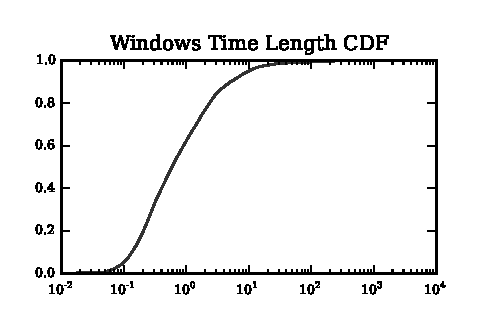
\includegraphics[scale=1]{./figures/window_time_size_histogram.eps}
\caption{Cumulative distribution function for the time length of the windows given in hours. Most windows' lengths are in the interval $[10^{-1}, 10^1]$ hours; about 60\% of windows are 1 hour or less, meaning users receive on average over 100 tweets an hour.}
\label{fig:window_time_size_histogram}
\end{figure}

\subsection{How prevalent are non-explicit responses?}

This section addresses the first research question \ref{rq:similarityPotential} of whether or not text similarity has potential for identifying untagged responses, starting with whether Tagged reactions indeed tend to have higher scores than Non-Tagged ones. 

\begin{table}[!tb]
	\centering
	\fontsize{9pt}{10pt}\selectfont
		\begin{tabular}{l|c|c|c|}
			\cline{2-4}
												& Mean					& Median					& Std. \\ \hline 
			\multicolumn{1}{|l|}{Non-Tagged}	& \nonTaggedScoreMean{}	&	\nonTaggedScoreMedian{}	& \nonTaggedScoreStd{} \\ \hline
			\multicolumn{1}{|l|}{Replies}		& \repliesScoreMean{}	&	\repliesScoreMedian{}	& \repliesScoreStd{} \\ \hline
			\multicolumn{1}{|l|}{Retweets}		& \retweetsScoreMean{}	&	\retweetsScoreMedian{}	& \retweetsScoreStd{} \\ \hline
		\end{tabular}
\caption{Sample mean and standard deviation for the normalized similarity score for the Replies, Retweets, and Non-Tagged sets.}
	\label{tab:sampleDistributionsStatistics}
\end{table}

\begin{figure}[!htbp]
\centering
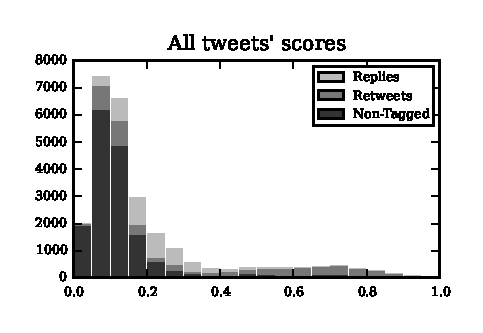
\includegraphics{./figures/all_tfidf_histogram.eps}
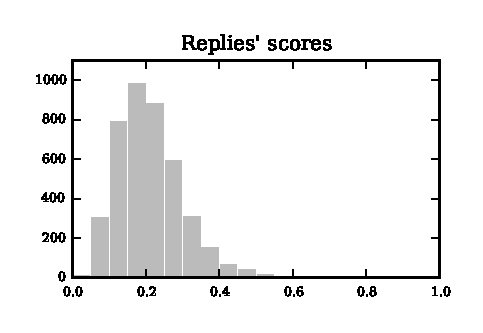
\includegraphics{./figures/replies_tfidf_histogram.eps}
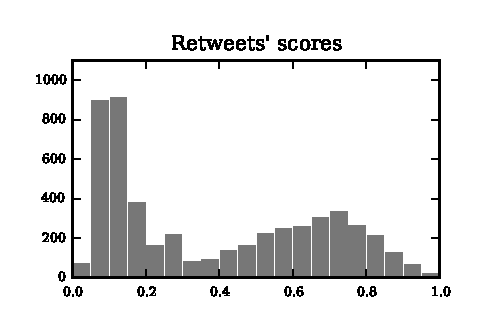
\includegraphics{./figures/retweets_tfidf_histogram.eps}
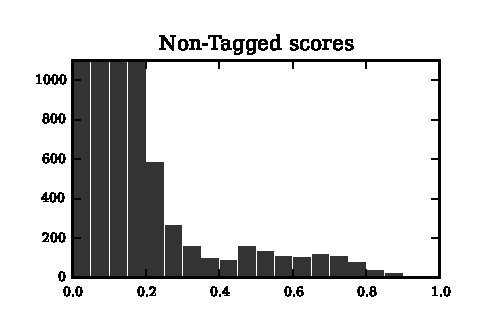
\includegraphics{./figures/not_retweets_replies_tfidf_histogram_cutoff_y.eps}
\caption{Histograms for the normalized similarity scores.  Note that the y-axis for the Non-Tagged subgraph was truncated at 1100 for better visualization of the tail of the distribution and matching other scales.  Retweets have a higher average score than Replies, which in turn are higher than Non-Tagged.  Further, Retweets have a bimodal distribution; high scores are near-duplicates of the tweets they are responding to, but over \lowRetweetCountPct{}\% have a score below \thresholdScore{}, suggesting that people often substantially edit retweets or retweet items not in their feed windows.}
\label{fig:fig_tweets_histograms}
\end{figure}

Mean and median scores are lowest for Non-Tagged and highest for Retweets, as shown in Table \ref{tab:sampleDistributionsStatistics}. This can also be seen in the scores' histogram for each of these sets in Figure \ref{fig:fig_tweets_histograms}. The score behaves as expected when we consider the averages, returning higher values for Replies and Retweets. However, the proximity of the means for the Replies and Non-Tagged and the higher variance of the Non-Tagged makes these two distributions not so well distinguishable based on score alone. The Retweets, on the other hand, present a heavier tail on the distribution. This suggests that the score captures general trends of the Tagged tweets, but is more suitable for Retweets. Considering that the Retweet average is \thresholdScore{} and that it is higher than the Replies mean by more than one standard deviation, \textbf{high scored messages} are defined as messages with $score \geq \thresholdScore{}$.
%% DC 26: It would be pretty straightforward to run something like a chi-square test to argue that the distributions are or are not significantly different (where you talk about "not so well distinguishable")

Although the Non-Tagged set has a lower average, it has a higher variance than replies. This comes from the fact that Non-Tagged tweets have a heavier tail when compared to replies, as seen in Figure \ref{fig:fig_tweets_histograms}. Also, the Non-Tagged high scored tweets are not neglectable when compared with the number of high scored Tagged tweets, as seen in Table \ref{tab:highScoredCounts}: such Non-Tagged tweets would comprise about \highNonTaggedTweetCountPct{}\% of responses, even with a fairly conservative cutoff of \thresholdScore{}. However, high scored messages misses most of the explicit Replies with this cutoff choice.

\begin{table}[!tb]
	\centering
	\fontsize{9pt}{11pt}\selectfont
		\begin{tabular}{l|>{\centering\arraybackslash}m{1.6cm}|>{\centering\arraybackslash}m{1cm}|>{\centering\arraybackslash}m{1.1cm}|}
			\cline{2-4}
			& Non-Tagged & Replies & Retweets \\ \hline
			\multicolumn{1}{|p{2.2cm}|}{\parbox[top][22pt][c]{2.2cm}{High Scored\\($score \geq \thresholdScore{}$)}} & 
			\cellcolor{gray!25} \highNonTaggedTweetCount{} & \highRepliesTweetCount{} & \highRetweetsTweetCount{} \\ \hline
			\multicolumn{1}{|p{2.2cm}|}{Total} & 
			\totalNonTaggedTweetCount{} & \cellcolor{gray!25} \totalReplies{} & \cellcolor{gray!25} \totalRetweets{} \\ \hline
		\end{tabular}
		\caption{Number of high scored messages and the total of messages for the sets Non-Tagged, Replies and Retweets. The highlighted number of high scored Non-Tagged messages is around \highNonTaggedTweetCountPct{}\% of the highlighted total of Tagged messages.}
	\label{tab:highScoredCounts}
\end{table}

Considering the retweet behavior, it would be expected that the normalized similarity score for retweeted messages would be high as long as the original tweet showed up in the windows and the retweet is basically reproducing the message with almost no modifications. 
Surprisingly, this is not what is observed in Figure \ref{fig:fig_tweets_histograms}.  Instead, more than \lowRetweetCountPct{}\% of Retweets have a $score < \thresholdScore{}$.  One possible explanation for this is that people sometimes retweet when they use other parts of the interface, such as other users' profiles or search results, or use social media share buttons attached to tweets on other sites.  Another possibility is that people might frequently edit retweets.

\subsection{Features of Replies, Retweets and Non-Tagged messages}

To help understand the mystery of low-scoring retweets, and more generally to understand what sorts of markers the method is using to identify potential responses, a sample of representative tweets from each category across a range of normalized similarity scores is examined.  
Tables \ref{tab:tweetsScoresRetweets}, \ref{tab:tweetsScoresReplies} and \ref{tab:tweetsScoresNonTagged} (see the Appendix) show both the user's tweet (top in each pair) and the text of the highest-scoring followee's tweet in the window for that tweet (bottom in each pair).

For system tagged Retweets, most of the high scored content has almost the same content as the original message (as expected), as in tweets \#1 and \#2 in the table.  One interesting thing to notice here is that as the tweet length decreases, the normalized similarity score goes down (compare \#6 to \#1). This is related to the fact that the $tf\mhyphen idf$ score is sensitive to the number of matched words between the query and the document.  
Below a threshold of around $0.3$ in this dataset, this effect disappears.  Instead, the text starts to look more like 
two tweets about a common external topic (\#7, \#8, \#9)---despite the fact that the tweet text preserves the ``RT'' retweet marker.  These would be likely candidates for actual retweets that occur outside the window, either farther back in the feed or other parts of the interface than the feed.

When looking at system tagged Replies, high-scoring replies show two main patterns.  In one, they look largely like retweets that were tagged as replies, likely because people pressed the reply button and pasted text from the text they replied to, as in \#11.  In the other, the tweet mentions multiple users who are conducting an ongoing conversation and want all of them to be notified when someone posts something new, as in \#12 and \#13.  It is important to notice that this set of tweets has a maximum score lower than the other sets; scores on the higher end of the distribution could not be found. Also, it appears that @-mentions are the main source of evidence for the normalized similarity scoring even as it goes down, and in fact, replies with low scores still often look like replies despite the low $tf\mhyphen idf$.  This is often (\#16, \#19) but not always (\#18, \#20) indicated by bi-directional @-mentions of the conversational partner.

When looking at Non-Tagged tweets, one of the first things to notice is that high scored tweets usually are retweets that were not captured by the system.  In some cases it is likely users are manually copying the content of the messages and adding retweet markers (\#23, \#24); in others, it is more likely that both users are independently retweeting external content (\#21, \#22).  Users often make small comments together with the original text (\#22, \#23, \#25).  As the normalized similarity score goes down, the messages look less like a retweet, but often still appear to be topically related, sometimes via hashtags (\#28, \#29).  

In general, higher normalized similarity scores seem to capture retweets reasonably well, even though being sensitive to their length, and a particular type of reply that involves conversations.  Non-tagged tweets with high scores are often retweets or quotes with extra comments from the users, although sometimes the retweets may be common retweeting of external content rather than retweets from the window.
%% DC 16: I don't really believe the following argument: #21 and 22 look much more like external stimulus to me.
%One initial concern about using text similarity was that it would be hard to distinguish actual responses from situations where people comment on a common external stimulus.  
%In these data, however, high scores appear to be reliably associated with responses rather than external stimulus.
Further, even the conservative estimate chosen shows that non-explicit responses are quite common---and it is likely that a number of the of the ``middle scoring'' tweets are actual responses.  Distinguishing those from external influences or underlying interest similarity would be an important next problem in building better models of non-explicit response.  

\subsection{Variations in User Responsiveness}

The previous sections demonstrate that it is likely that \highNonTaggedTweetCountPct{}\% or more of Non-Tagged tweets are responses that are not explicitly captured by the system.  This section addresses the other main research question \ref{rq:usersDistribution} of how these losses are distributed among different users in the network.   

These Non-Tagged high-scored messages were authored by \highUserCount{} of the \totalUsers{} users (\highUserCountPct{}\%). This suggests that users generate responses that are missed in a non-uniform way: many users behave as the system expects, using explicit reply and retweet mechanisms, but a significant number respond, at least sometimes, without using those mechanisms. 
Figure \ref{fig:users_reponse_histograms} shows histograms for example users that have most or all of their responses untagged by Twitter even though they present a high $score$.  Note that these users span a range of activity levels, meaning that they are not just newbies that do not know how to use the interface.

\begin{figure}[!tb]
\centering
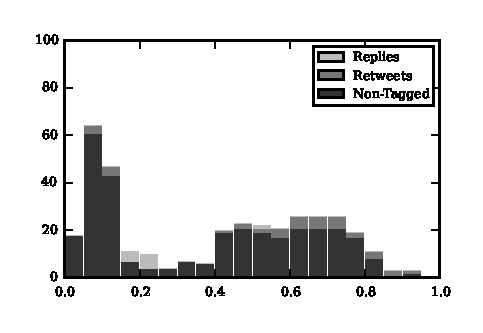
\includegraphics[scale=0.9]{./figures/213501392_histogram.eps}
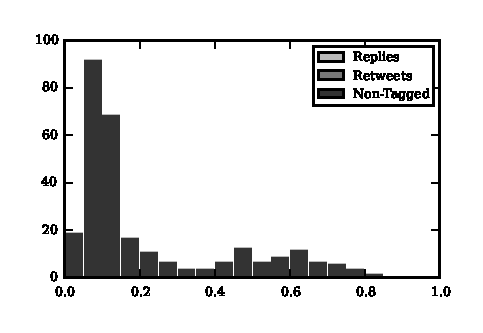
\includegraphics[scale=0.9]{./figures/808181892_histogram.eps}
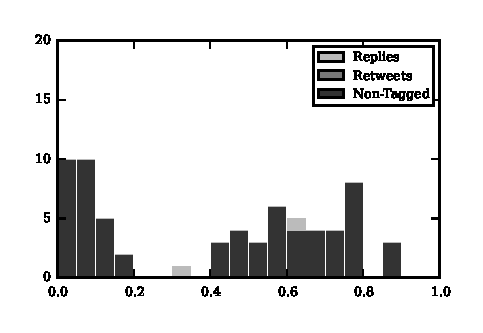
\includegraphics[scale=0.9]{./figures/87339782_histogram.eps}
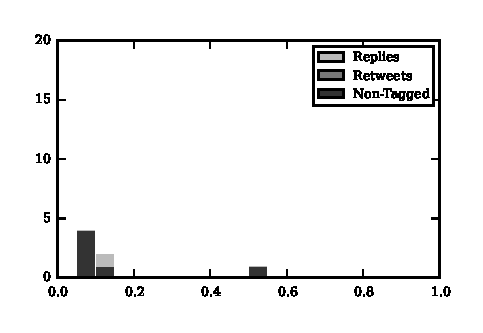
\includegraphics[scale=0.9]{./figures/196322186_histogram.eps}
\caption{Score histograms for sample users who present a significant amount of high scored Non-Tagged content relative to their total amount of messages, which indicates that most of their reactions are not being properly tagged by Twitter.}
\label{fig:users_reponse_histograms}
\end{figure}


In order to better understand the behavior distribution among all users, Figure \ref{fig:2d_histogram} shows a 2d-histogram for the points $(p_i^T, p_i^N)$, where each of these points is the percentage of the Tagged messages $p_i^T$ and the percentage of the high scored Non-Tagged messages $p_i^N$.  Each of these points is evaluated for a user $u_i$ in relation to the total number of messages the user authored.
The high scored Non-Tagged percentage $p_i^N$ is the proportion of this user behavior that were likely to be reactions while the percentage $p_i^T$ is the proportion of reactions actually captured.


The \usersScoreZero{} users that never have messages that scored higher than $\thresholdScore{}$ nor used explicit system reply mechanisms are concentrated at the origin of the histogram.
Users that lay on the $x$-axis only react through explicit reaction mechanisms the system offers, therefore have all their reaction Tagged. Similarly, users on the $y$-axis never use explicit reaction mechanisms, although they present high scored Non-Tagged content. Users above the dashed line have more high scored Non-Tagged content than Tagged content. It is possible to say that users that lay above the dashed line are more likely to produce content that can be missed by Twitter's tagging system, and they account for \usersAboveLine{} users, about $\usersAboveLinePct{}\%$ of the dataset. 

\begin{figure}[!tb]
\centering
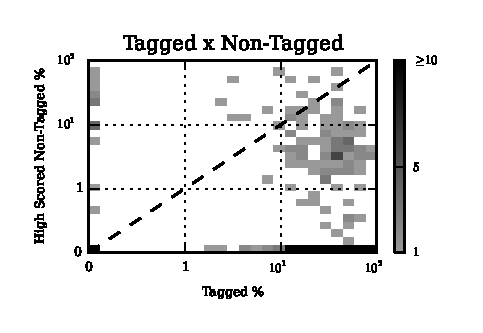
\includegraphics[scale=1.2]{./figures/user_alltagged_highnontagged_2dhist_0375.eps}
\caption{2D histogram of the percentage of Tagged and high-scored Non-Tagged messages for all users. The scale is linear in the interval $[0,1]$ and logarithmic on the interval $(1,100]$; the dashed line represents an equal percentage of Tagged and Non-Tagged tweets. 
Many users are non-responsive (the point at the origin) or use the explicit response mechanisms consistently (points hugging the x-axis with a 0 value for high scored Non-Tagged \%).  However, a significant number never use the explicit response mechanisms (points hugging the y-axis with a 0 value for Tagged \%), use them only occasionally (points above the dashed line), or occasionally forget to use them (points below the dashed line).}
\label{fig:2d_histogram}
\end{figure}


\begin{figure}[!tb]
\centering
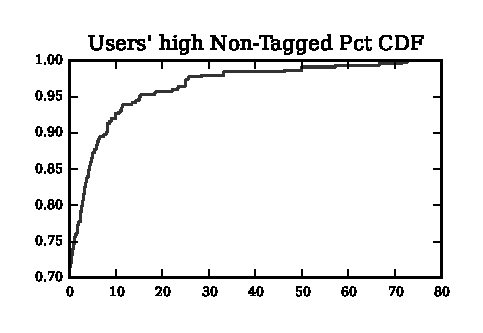
\includegraphics[scale=1]{./figures/users_high_nontagged_pct_cdf.eps}
\caption{Cumulative distribution of the users for the percentage of high scored Non-Tagged messages. \usersZeroHighScoredPct{}\% of the users have no high scored Non-Tagged messages, while \usersMoreThanTenPctPct{}\% of the users had at least 10\% of their messages high scored and Non-Tagged.}
\label{fig:cumulative_user}
\end{figure}


When considering the cumulative distribution of the users according to the percentage of high scored Non-Tagged messages $p_i^N$, shown in Figure \ref{fig:cumulative_user}, we identify more than \usersMoreThanTenPctPct{}\% of the users with at least 10\% of their messages being high scored and missed by Twitter's tagging system. 

These results indicate that methods that rely on explicit indicators of response likely miss or seriously under-represent the behavior of a sizable proportion of the Twitter population.


\subsection{Manual Retweeting}

A significant number of high scored messages identified by our method were actual retweets that were not tagged by the system, meaning that users actually copied and pasted the original tweet in order to produce these particular retweets (often adding extra comments of their own). This is actually a common practice advised by online marketeers to increase reach and visibility of one's retweets \cite{ManualRetweet1, ManualRetweet2, ManualRetweet3}. Their main arguments is that the built-in retweets suffer a series of shortcomings: they lack the possibility of being edited by the retweeting user, followers can set their feed to filter out built-in retweets, trackings for the link interactions for a built-in retweet are attributed to the original post link only, lack of information about who retweeted, since it shows more information about the original poster. These issues might be reason enough to explain why we see more than \usersMoreThanTenPctPct{}\% of users putting on the extra effort of manually coping and pasting, as well as editing the original message, in order to avoid these shortcomings of the built-in retweets.

\subsection{Implicit Response Detection Through Provenance}

Information provenance is a related field to the work presented here. Its main goal is to establish the origin of a given content. It can be useful to asses influence and trustworthiness, for instance. It is also interpreted as the reverse process of information diffusion \cite{taxidou2015}.

A relevant provenance model that is closely related to our work was published later by De Nies et al. \cite{de2015}. It uses a multi-level provenance method, and one of its steps to cluster messages in a tf-idf feature space. The clustering method chooses an arbitrary threshold that is closely related to the cluster size (higher thresholds lead to smaller clusters and vice-versa). For each cluster, the oldest message is said to be the root message of the cluster, and all the messages in the cluster share some provenance with it. This method was later used by Taxidou et al. \cite{taxidou2016} to infer implicit interactions. Their work defined three possible types of interaction, which included subtypes: 1) user influence: a) with explicit credit, b) without credit, 2) external influence, 3) self-influence: a) delete and rewrite, b) promotion. From a total of 3909 messages, they found that explicit interactions were 2068 retweets, 198 quotes, and 93 replies, for a total of 2359 Tagged messages. Using the tf-idf similarity method and a threshold of 0.4 (for which they claim that messages above this similarity are likely to share some provenance), they detected another 192 messages that shared provenance but were not explicit Tagged. Using the same relative analysis as we did in our work, the implicit interactions represents about 8.1\% of the total of explicit interactions.

When comparing our results, we should bear in mind that there are limitations to how these methods work and the datasets that were used. Their method takes a full dataset and cluster over all its messages, in contrast to our approach that is user-centered. Their dataset was crawled from the Twitter streaming API based on keywords related to the ISWC 2015 conference, therefore it is biased to this topic. In our dataset, we chose a set of users that followed Obama and crawled all their ego-network tweets, reducing possible biases since the bias would be in the choice of the user and not of the messages. Also, since it is not a user-centered approach, all analysis are comparable only at the message level, not allowing us to compare user's profiles and patterns of behavior. Finally, they considered quotes as an explicit reaction (which was included in the 8.1\% previously mentioned), while our method only considered replies and retweets.

Regardless of these limitations, the fact that the underlying method uses tf-idf to evaluate similarity over tweets and identifies implicit reactions allow us to compare results. In our method, we identified \highNonTaggedTweetCountPct{}\% of the Non-Tagged tweets as possible reactions in comparison with the Tagged ones, opposed to 8.1\% using their method. We can attribute this difference to the fact that our model takes into consideration a more specific baseline of comparison, since we calculate new tf-idf scores for each ego-network. Also, we used a different threshold for our score, which could yield these differences. Nevertheless, their results are in line with our first research question \ref{rq:similarityPotential}. It supports the claim that text similarity has the potential to detect implicit responses and presents estimates for theses numbers that are within the same order of magnitude of our results.


\section{Contributions}

This chapter presented a novel method for user's non-explicit reactions to followees' content detection in Twitter. It is based on text similarity scores between a user's tweets and those of their followees \cite{Barbosa}.  Our method generates higher scores on average for system tagged Replies and Retweets than Non-Tagged tweets, suggesting that our text similarity scores have the potential to identify users' reactions as stated in our first research question \ref{rq:similarityPotential}.  

When using a conservative cutoff to detect non-tagged reactions, our results indicate that at least \highNonTaggedTweetCountPct{}\% of users' reactions are not tagged by the system.  Considering our second research question \ref{rq:usersDistribution}, almost a quarter of the users in our dataset presented non-tagged reactions. Furthermore, among these users we have another quarter of them exhibiting more missed reactions than explicit system tagged ones. These users have a wide range of activity level, with dozens or hundreds of tweets in a 14-day window, meaning that they are not just naive, low-activity users who do not understand Twitter.

\subsection{Limitations and future work}

The pattern of behavior of each individual is taken into account in this work when we consider each users' ego-network for our model. However, we modeled reactions in a broad meaning: users could be reacting to each other, or reacting to a common external event or even just posting the same thing by coincidence. While all these effects are interesting and we would like to be able to distinguish users in these dimensions -- users that have a high reaction rate to other users might be interesting as followers. Users that are prone to react to certain external events might be interesting as a target audience for these events. Users that just happen to post the same things might be clustered together for marketing campaigns. Our method as designed does not account for these differences. Once we detect a reaction, we could further refine it in these dimensions and have a more fine grained model of each user. This would be a natural development of this model.

Another important aspect that we did not consider here is that text is not everything. Nowadays more than ever, images and videos are commonly used in social networks posts and they carry a significant amount of information. Mapping and understanding how users react to this content could improve our method, and researchers such as Cavalin et al. \cite{Cavalin2016} have been working in tools to better aggregate and understand Twitter posts that contain images.

